
\section{Results and Discussion}
% Describe evaluation methodology and significant results in the evaluation section
% Evaluate the selected approach and analyze why the selected approach is good?
%   Provide an intuitive description of the algorithms, their correctness and their complexity
\subsection{Simulation Overview}
The simulation was run
on a Dell Laptop with a 11th Gen Intel(R) Core(TM) i7-11800H processor (8 cores, 16 threads)
running at 2.30GHz, 64.0 GB of installed RAM,
a 64-bit operating system with an x64-based processor
using Python3.10 and pytest as the driver.
We selected Pytest because the test-isolation generalizes
well for simulations. Therefore, simulations
are `tests' marked with the \texttt{@pytest.mark.simulation}
marker. Because running a simulation is slow,
these tests are also marked as \textit{slow}.

More importantly, we run our simulation
distributed across multiple CPUs. Given that
each simulation is isolated, we can run
all the simulations in parallel
by using pytest-xdist framework~\cite{pytestXdist}.
Additionally, pytest ships with runtime
tracking out of the box.
Refer to \autoref{fig:simulation}
for an example output of a running simulation.

\begin{figure}[!htp]
    \centering
    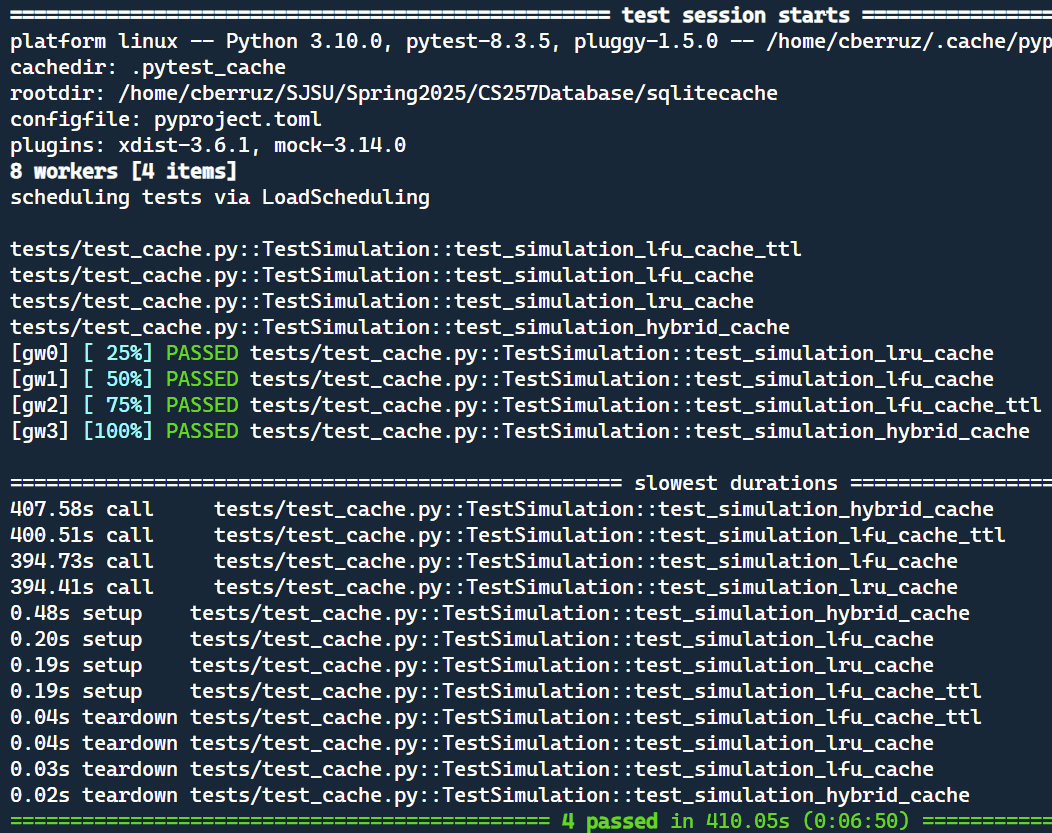
\includegraphics[width=\linewidth]{images/simulation_running_example.png}
    \caption{Screenshot of a running simulation.}
    \label{fig:simulation}
\end{figure}

\subsection{Simulation Details}
We let $P = 100$.
In our platform, all uncompressed and unencrypted
values in $D$ occupy $b = 18$ bytes.
Therefore, the cache size $P' = Q' = 1800$ bytes.
Furthermore, no compression and no encryption
was enabled.

The simulation was run as a sustained load
with $N = 100,000$ requests,
as described in Algorithm~\ref{alg:simulation}.
This means that the simulation runs until completion
for
$N$ requests. For example, in $N=1000$
we generate 1000 data points for both
the hit and miss rates. The duration
of each simulation run was dependent
on the eviction policy being tested.
TTL based policies, such as LFUCacheTTL
and HybridCache
took the longest. Please refer to \autoref{tab:test_simulation_metrics}
for a detailed view of the runtime of the simulations
depending on the eviction policy.

A total of four eviction policies were tested:
LRU, LFU, LFU with TTL, and Hybrid.
For any TTL based policy, we used a TTL of 5 seconds.
Finally, for the hybrid policy we set the threshold
$T = 5$. Recall that $T$ is a counter threshold
that dictates the number of times
and item is looked up before it is
moved from the LRUCache
into the LFUCache with TTL.

\subsection{Hit Rate analysis}
The results of the hit rate vs. the number
of request for each eviction policy is summarized
in \autoref{fig:hit_rate_plot}.

\begin{figure*}[!htp]
    \centering
    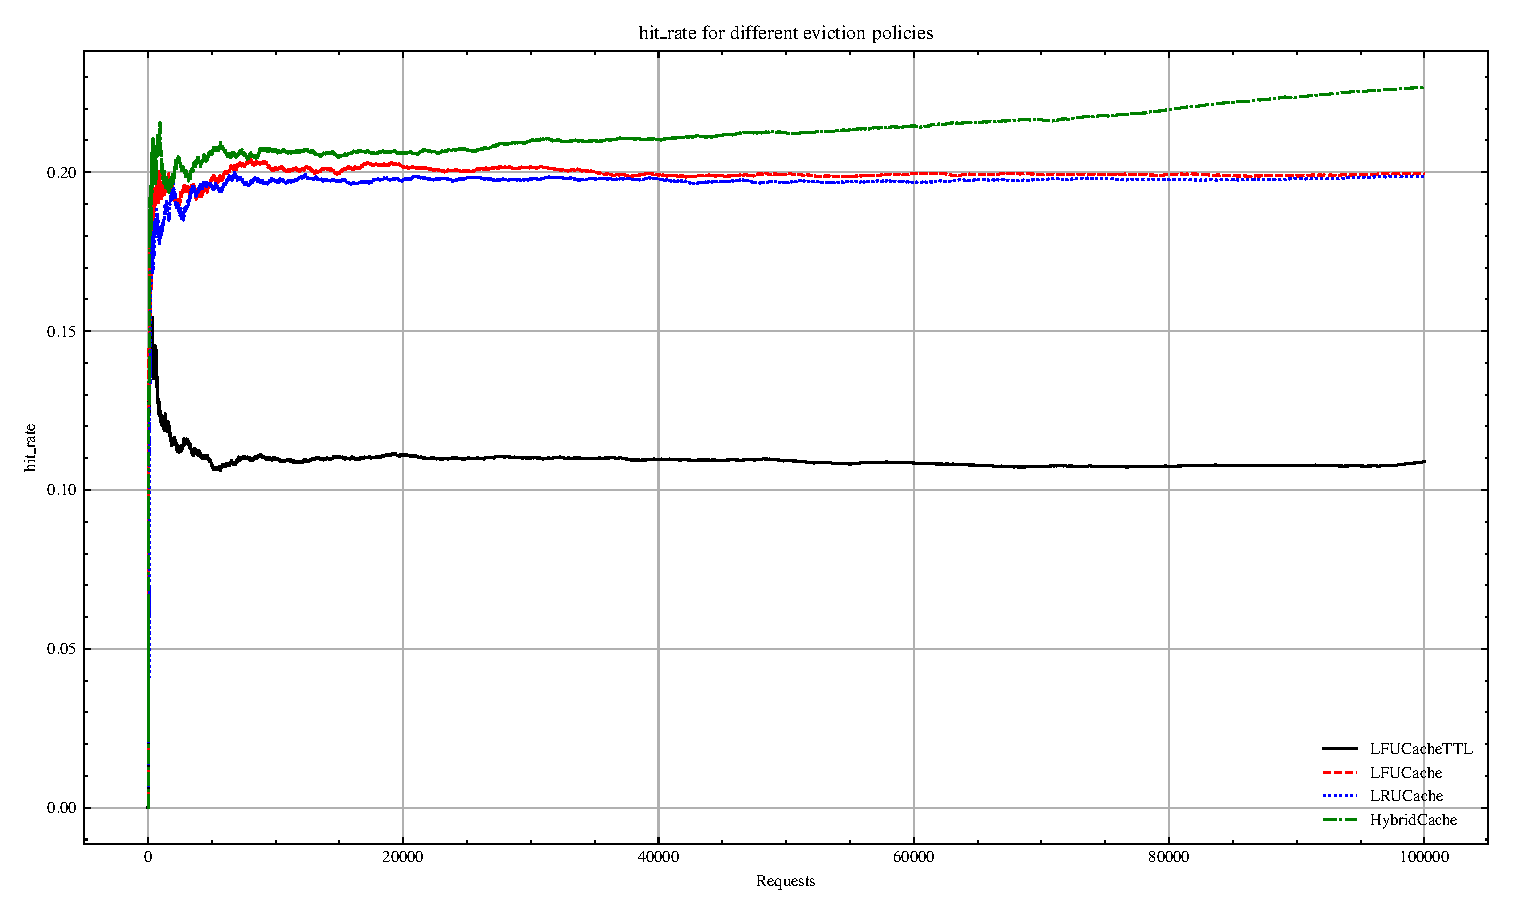
\includegraphics[width=\textwidth]{images/hit_rate_plot.eps} % Replace with the path to your EPS file
    \caption{Hit rate as a function of requests among different eviction policies}
    \label{fig:hit_rate_plot}
\end{figure*}

It is clear that the HybridCache policy performs significantly
better than all other policies across all number of requests.
The LFUCache with TTL performs the worst
among all eviction policies. These results
are in alignment with~\cite{shah2023ImprovedCacheEviction}.
Note that both the LRUCache and LFUCache eviction
policies converge at a hit rate of 20\%.
Interestingly, \[hit\_rate \approx 0.20 = \frac{100}{500} = \frac{P}{|D|}\]
which is a sign that caches converging
to $\frac{P}{|D|}$ do not generalize well as it
is the uniform random probability of selecting $P$ items
out of a set of size $|D|$.

It is important to note that our results do not
exactly match
the ones reported in~\cite{shah2023ImprovedCacheEviction}.
We believe this is due to two reasons:

\begin{enumerate}
    \item \textbf{True randomness:} our methodology explicitly
    describes that values selected from $D$ have the same
    probability of being selected. Authors in~\cite{shah2023ImprovedCacheEviction}
    do not specify the probabilities of items drawn from $D$.
    \item \textbf{I/O Cost:} The hybrid cache
    described in~\cite{shah2023ImprovedCacheEviction}
    makes the assumption that all data structures
    and data live in memory. Given that the HybridCache
    incurs runtime penalty due to I/O, this affects
    the underlying TTL eviction. Therefore,
    it is unrealistic to expect the same results.
\end{enumerate}

Finally, note that as the number of request increases, the
difference between the hit rate of the HybridCache
and all other cache increases. This is a great sign
that the eviction policy is able to adapt to unpredictable
(random)
workloads.

\subsection{Miss Rate Analysis}

\autoref{fig:miss_rate_plot} shows the miss rate as a function
of requests for all eviction policies.
Our miss rate is defined as
\[miss\_rate = 1 - hit\_rate\]

Note that by definition, \autoref{fig:miss_rate_plot}
is the inverse of \autoref{fig:hit_rate_plot}. 
One thing to point out is that at the beginning
of the simulation, the miss rate is incredibly high.
This makes sense because at the beginning of the simulation,
the number of elements that can be possibly looked up
is significantly greater than the number of elements
currently in the cache. For example, if only
one element is currently in the cache,
the probability of that element \textbf{not being selected}
for a lookup in the cache is \[\frac{499}{500} = 0.998\].

Similar to the hit rate, the miss rate stabilizes
for most cache classes. Furthermore, the HybridCache
sees a reduction of the miss rate as the
number of requests increases \textemdash~validating
our hypothesis of adaptability.

\begin{figure*}[!htp]
    \centering
    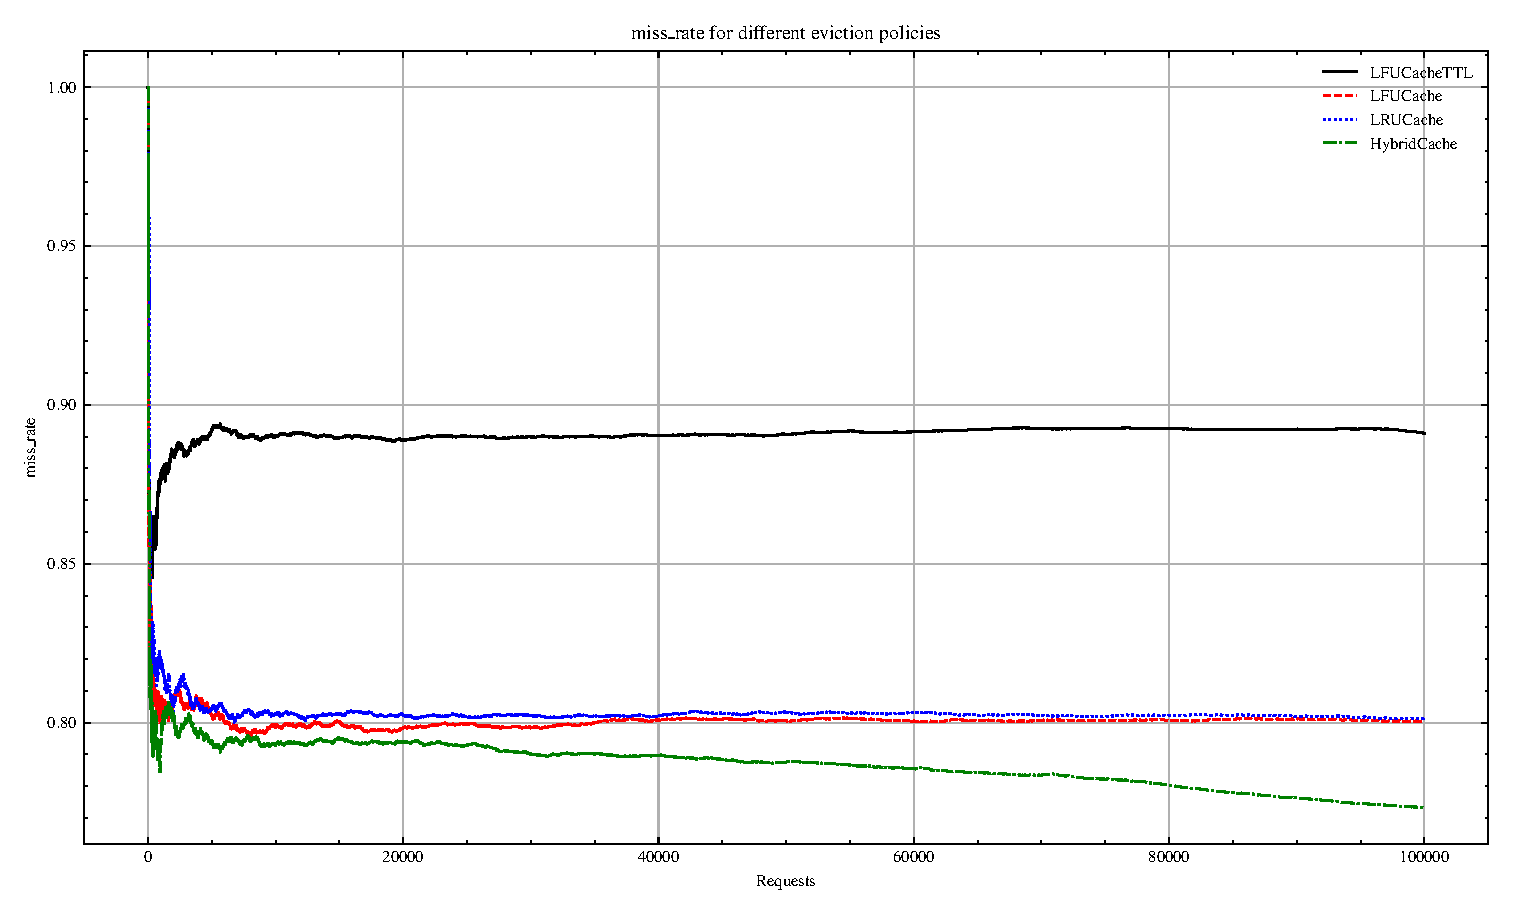
\includegraphics[width=\textwidth]{images/miss_rate_plot.eps} % Replace with the path to your EPS file
    \caption{Hit rate as a function of requests among different eviction policies}
    \label{fig:miss_rate_plot}
\end{figure*}

\subsection{Runtime Analysis}
Given the persistency of all our cache implementations,
it is worth to discuss the runtime differences among
them. \autoref{tab:test_simulation_metrics} summarizes
the runtime of the simulation for all the eviction policies.

\begin{table}[!htp]
    \centering
    \caption{Runtime metrics for different simulations with 100,000 requests}
    \label{tab:test_simulation_metrics}
    \begin{tabularx}{\linewidth}{XXX}
        \toprule
        \textbf{Cache} & \textbf{Runtime (s)} & \textbf{Runtime (h)} \\
        \midrule
        HybridCache & 8484.57 & 2.36 \\
        LFUCache (TTL) & 8339.01 & 2.32 \\
        LRUCache & 8190.93 & 2.28 \\
        LFUCache & 8169.70 & 2.27 \\
        \bottomrule
    \end{tabularx}
\end{table}

As expected, TTL based policies such as LFUCache with TTL,
and the HybridCache have the longest runtime. However,
when compared with the lowest runtime, these two
policies are only 2\% and 4\% slower, respectively.
Therefore, we can argue that our choice of in-demand
eviction of expired items was a smart design choice
because the runtime penalty is minimal.